\graphicspath{{2trig/asy/}}

\section{Trigonometric Functions and Polar Co-ordinates}\label{sec:trig}

In this chapter we review trigonometry and periodic functions and discuss their relation to polar co-ordinates. Some of this will be non-standard.

\subsection{Definitions \& Measuring Angles}\label{ssec:trigdef}

\begin{minipage}[t]{0.74\linewidth}\vspace{-5pt}
	Trigonometric functions date back at least 2000 years. Ancient mathematicians were interested in the relationship between the \emph{chord} of a circle and the central angle, often for the purpose of astronomical measurement. It wasn't until 1595 that the term \emph{trigonometry} (literally \emph{triangle measure}) was coined, and the functions were considered as coming from triangles.
\end{minipage}
\hfill
\begin{minipage}[t]{0.25\linewidth}\vspace{-15pt}
	\flushright
	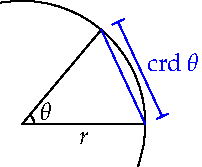
\includegraphics{defn-chord}
\end{minipage}
\smallbreak

Here are several related definitions of sine, cosine and tangent based either on triangles or circles.


\begin{defn}[lower separated=false, sidebyside, sidebyside align=top seam, sidebyside gap=0pt, righthand width=0.28\linewidth]{}{polarcoord}
	\hangindent\doubleind
	1.\lstsp(a)\lstsp Given a right triangle with \emph{hypotenuse} (longest side) 1 and angle $\theta$, define $\textcolor{blue}{\sin\theta}$ and $\textcolor{Green}{\cos\theta}$ to be the side lengths \emph{opposite} and \emph{adjacent} to $\theta$.\vspace{-5pt}
	\begin{enumerate}\setcounter{enumi}{1} 
	  \item[]
	  \begin{enumerate}\setcounter{enumii}{1}
	    \item[] Define $\tan\theta=\frac{\sin\theta}{\cos\theta}$ to be the slope of the hypotenuse.
	    \item Given a right triangle with angle $\theta$, \emph{hypotenuse} $r$, \emph{adjacent} $x$ and \emph{opposite} $y$, define
			\[
				\sin\theta=\frac yr\qquad \cos\theta=\frac xr\qquad \tan\theta=\frac yx
			\]
	  \end{enumerate}\vspace{-8pt}
	  \item\begin{enumerate}
	    \item $(\cos\theta,\sin\theta)$ are the co-ordinates of a point on the unit circle, where $\theta$ is its \emph{polar angle} measured counter-clockwise from the positive $x$-axis. Provided $\cos\theta\neq 0$, also define $\tan\theta=\frac{\sin\theta}{\cos\theta}$.
	    \item Repeat the definition for a circle of radius $r$ with co-ordinates $(r\cos\theta,r\sin\theta)$.
	  \end{enumerate}
	\end{enumerate}
	\tcblower
	\flushright
	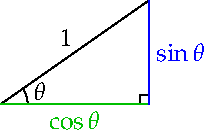
\includegraphics{defn-trig1}\par
	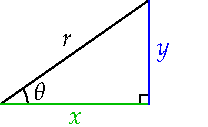
\includegraphics{defn-trig2}\par
	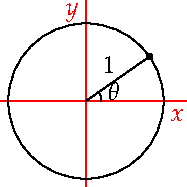
\includegraphics{defn-trig3}\phantom{bobo}
\end{defn}

Discuss some of the advantages and weaknesses of these definitions:
\begin{itemize}
  \item What prerequisites are you assuming in each case?
  \item Is it easier to think about \emph{lengths} rather than ratios?
  \item Where do you need basic facts from Euclidean geometry such as \emph{congruent/similar} triangles?
  \item Convince yourself that that the triangle definitions follow from the circle definitions. What is missing if you try to use the triangle definition to justify the circle version?
  \item If you were introducing trigonometry for the first time, what would you use?
\end{itemize}
If you've done sufficient calculus you might know of other definitions, for instance using power (Maclaurin) series. Plainly these are not suitable for grade-school, but have the great benefit of making the calculus relationship $\diff\theta\sin\theta=\cos\theta$ very simple. Establishing this using the triangle definition is a somewhat tricky!


\boldsubsubsection{Measuring Angles}

There are two standard ways to measure angles (to sensibly associate a \emph{number} to each angle).

\begin{description}
	\item[\normalfont\emph{Degrees}] A full revolution has \ang{360} and a right-angle \ang{90}. Degree measure dates back to ancient Babylon 2--4000 years ago.\footnote{%
	It is not known why they chose 360, but it fits nicely with their \emph{base-60} system of counting (decimals are base-10). The traditional subdivisions of a degree are also base-60. For instance, $\ang{34}12'45"$ is 34 degrees, 12 (arc)minutes and 45 (arc)seconds; converted to decimal notation, this becomes
	\[
		\ang{34}12'45" =34+\frac{12}{60}+\frac{45}{60^2}=\ang{34.2125}
	\]
	The standard hour-minute-second measurement of time has the same origin.%
}


	\item[\normalfont\emph{Radians}] The radian measure of an angle is the \textcolor{blue}{length of the arc} subtending the angle in a circle of radius 1. Since the circumference of a unit circle is $2\pi$, we have the following identifications.\par
	\begin{minipage}[t]{0.59\linewidth}\vspace{-18pt}
		\[
			\def\arraystretch{1.1}
			\begin{array}{c|c|c|c|c}
				\text{Degrees}&\text{Radians}&\sin\theta&\cos\theta&\tan\theta\\\hline
				\ang{0}&0&0&1&0\\
				\ang{30}&\frac\pi 6&\frac 12&\frac{\sqrt 3}2&\frac 1{\sqrt 3}\\
				\ang{45}&\frac\pi 4&\frac 1{\sqrt 2}&\frac 1{\sqrt 2}&1\\
				\ang{60}&\frac\pi 3&\frac{\sqrt 3}2&\frac 12&\sqrt 3\\
				\ang{90}&\frac\pi 2&1&0&\text{n/a}\\
				\ang{180}&\pi&0&-1&0
			\end{array}
		\]
	\end{minipage}
	\hfill
	\begin{minipage}[t]{0.4\linewidth}\vspace{-10pt}
		\flushright
		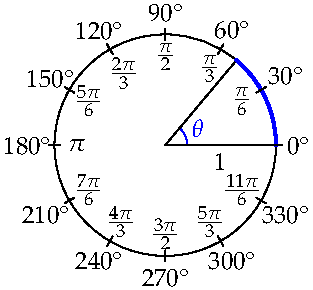
\includegraphics[scale=0.95]{defn-radians}
	\end{minipage}
\end{description}

In elementary mathematics, degrees are the most common way to measure angles. Do you know any other methods?

\begin{exercises}
	\exstart The identity $\cos^2\!\theta+\sin^2\!\theta=1$ is the Pythagorean Theorem in disguise. Why?
	
	\begin{enumerate}\setcounter{enumi}{1}
	  \item The word \emph{sine} is the result of a long list of translations and transliterations from an ancient Sanskrit term meaning \emph{half-chord.} For the chord picture on page \pageref{sec:trig}, how does the length of the chord $\operatorname{crd}\theta$ relate to modern trigonometric functions?
	
		\item It is conventional not to state units when using radians since they are effectively a ratio and therefore \emph{unitless.} Think this through: if the central angle in a circle of radius $r$ is subtended by an arc with arc-length $\ell$, what is the radian measure of the angle? What facts from Euclidean geometry justify this observation?
		
	  \item Explain how to get the values of sine and cosine in the above table.\par
	  (\emph{Hint: Draw some triangles and use Pythagoras}!)
	  
	  \item\label{exs:trigshift} Using the pictures, explain why we have the relations
		\[
			\sin(\tfrac \pi 2-\theta)=\cos\theta=\sin(\theta+\tfrac\pi 2),
			\qquad 
			\sin(-\theta)=-\sin\theta,\qquad \sin(\pi-\theta)=\sin\theta
			\]
		(\emph{You cannot use multiple-angle formulæ for this!})
	\end{enumerate}
\end{exercises}


\clearpage


\subsection{Periodicity, Graphs \& Inverses}\label{ssec:trigperiod}

One advantage of the circle definition is that it makes sketching the graphs of sine and cosine very easy. Simply draw axes next to a unit circle and transfer the heights across.
\begin{center}
	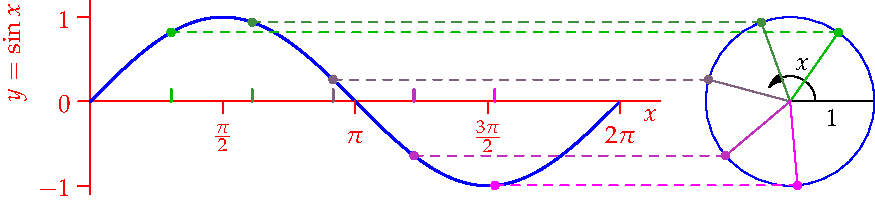
\includegraphics{invsine4}
\end{center}
By Exercise \ref*{ssec:trigdef}.\ref{exs:trigshift}, the graph of $\cos x=\sin(x+\frac\pi 2)$ is simply that of sine shifted $\frac\pi 2=\ang{90}$ to the left. Moreover, the circle definition allows us easily to extend trigonometric functions \emph{periodically} since we can measure the polar angle by looping as many times round the origin as we like: for any integer $n$,
\[
	\sin(\theta+2n\pi)=\sin\theta,\quad 
	\cos(\theta+2n\pi)=\cos\theta
\]
Otherwise said, sine and cosine have period $2\pi$ radians ($\ang{360}$).\medbreak


Sine and cosine are \emph{non-invertible} unless we choose a domain on which they are 1--1.\par
\begin{minipage}[t]{0.6\textwidth}\vspace{-3pt}
	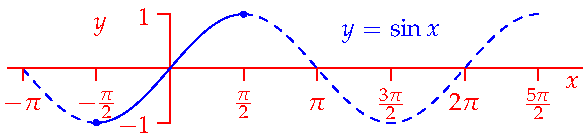
\includegraphics[scale=0.95]{invsine2}\par
	$f(x)=\sin x$ is 1--1 on the domain $[-\frac\pi 2,\frac\pi 2]$\smallbreak
	Inverse function $f^{-1}(x)=\arcsin x=\sin^{-1}x$\smallbreak
	Domain $\dom(\arcsin)=[-1,1] =\operatorname{range}(\sin)$\smallbreak
	Range $\operatorname{range}(\arcsin)=[-\frac\pi 2,\frac\pi 2]=\dom(\sin)$\medbreak
	This is why your calculator always returns a value in the interval $[-\frac\pi 2,\frac\pi 2]=[-\ang{90},\ang{90}]$ when you hit the $\sin^{-1}$ button.
\end{minipage}
\hfill
\begin{minipage}[t]{0.39\textwidth}\vspace{-5pt}
	\flushright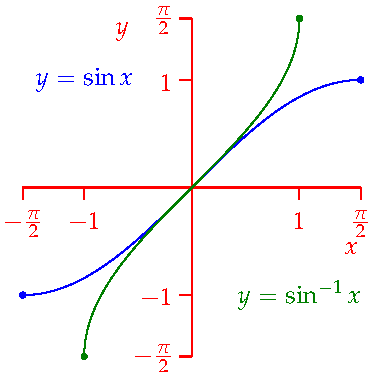
\includegraphics[scale=0.9]{invsine}
\end{minipage}

\begin{example}{}{sineeasy}
	If you know the graphs, then symmetry and periodicity help you solve equations. For example, if $\sin \theta=\frac 9{10}$ then all solutions are given by
	\[
		\theta=\sin^{-1}\frac 9{10}+2\pi n
		\quad\text{or}\quad 
		\pi-\sin^{-1}\frac 9{10}+2\pi n \tag{$n$ is any integer}
	\]
	\begin{center}
		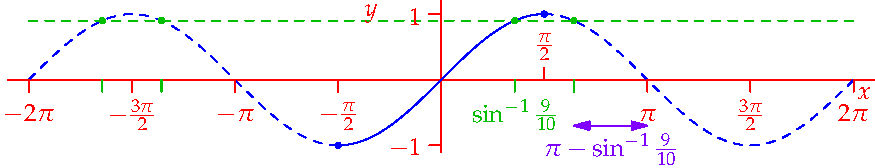
\includegraphics[scale=0.95]{invsine3}
	\end{center}
	Alternatively, we could use the circle definition directly: $\sin\theta=\frac 9{10}$ means we want angles $\theta$ corresponding to the intersections of the unit circle with the \emph{horizontal line} $y=\frac 9{10}$.
\end{example}


\goodbreak


\boldinline{Periodic Models}

Trig functions find applications in modeling precisely because they are \emph{periodic.} In general, a function has period $T$ if
\[
	f(x+T)=f(x)\ \text{ for all $x$}
\]
It is easy to find the period of the function $f(x)=\sin kx$ just by considering what we have to add to the input $x$ to increase the argument $kx$ of sine by $2\pi$:
\[
	T=\frac{2\pi}k\implies f(x+T)=\sin(kx+2\pi)=\sin kx=f(x)
\]
We may therefore obtain a simple periodic model regardless of what period is required.

\begin{example}{}{}
	On a given day, \textcolor{Magenta}{high tide} occurs at 2:00 with a water depth of 10\,ft, whereas \textcolor{Green}{low tide} occurs at 8:12 with a depth of 4\,ft. We might model this using a periodic function with period $T=2\times 6\frac{12}{60}=\frac{62}{5}$ hours. For instance\par
	\begin{minipage}[t]{0.6\linewidth}\vspace{-8pt}
		\[
			h(t)=7+3\cos\left(\frac{5\pi}{31}(t-4)\right)
		\] 
	\end{minipage}
	\hfill
	\begin{minipage}[t]{0.39\linewidth}\vspace{-18pt}
		\flushright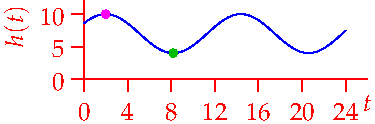
\includegraphics{tide}
	\end{minipage}\medbreak
	where $t$ is measured in hours from midnight might be suitable. In reality, tidal height is very close to being periodic, but the magnitude of the high and low tides are somewhat variable.
\end{example}


In fact \emph{any} periodic function may be approximated using trigonometric functions. Indeed if $f(x)$ has period $T$ and we define constants
\[
	a_n=\int_{-\frac T2}^{\frac T2} f(x)\cos\frac{2\pi nx}T\,\dx,\qquad 
	b_n=\int_{-\frac T2}^{\frac T2} f(x)\sin\frac{2\pi nx}T\,\dx
	\tag{$\ast$}
\]
then
\[
	f(x)\approx \frac{a_0}2+a_1\cos\frac{2\pi x}T +b_1\sin\frac{2\pi x}T +a_2\cos\frac{4\pi x}T +b_2\sin\frac{4\pi x}T +\cdots \tag{$\dag$}
\]
This is the \emph{Fourier series} of $f(x)$. It often takes only a small number of terms to obtain a very good approximation. Modern data-compression algorithms often employ Fourier series. Given a periodic function $f(x)$, one uses a computer to estimate (say) the first 100 Fourier coefficients ($\ast$) and transmits these values to the receiver, who recovers an approximation to the original function using $(\dag)$.

\begin{example}{}{}
	A square-wave function with period $T=2\pi$ is given by\par
	\begin{minipage}[t]{0.6\linewidth}\vspace{-10pt}
		\[
			f(x)=
			\begin{cases}
				1&\text{if }0\le x<\pi\\
				-1&\text{if }\pi\le x<2\pi
			\end{cases}
		\]
		extended periodically to the real line. With a little calculus, it is easily checked that the Fourier coefficients are
	\end{minipage}
	\hfill
	\begin{minipage}[t]{0.39\linewidth}\vspace{-2pt}
		\flushright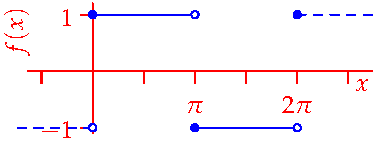
\includegraphics[scale=0.95]{square-wave}
	\end{minipage}\par
	\[
		a_n=\int_{-\pi}^{\pi} f(x)\cos nx\,\dx=0,\qquad 
		b_n=\int_{-\pi}^{\pi} f(x)\sin nx\,\dx=
		\begin{cases}
			\frac 4{\pi n}&\text{if $n$ is odd}\\
			0&\text{if $n$ is even}
		\end{cases}
	\]
	Use a graphics tool to see how the first few terms of the series \href{https://www.math.uci.edu/~ndonalds/math121b/orth-fourier.html}{approximate the function.}
\end{example}


\goodbreak


\begin{exercises}
	\exstart $f(x)=\sin x$ is also 1--1 on the interval $[\frac\pi 2,\frac{3\pi}2]$. Sketch the graph of its corresponding inverse function.
	
	\begin{enumerate}\setcounter{enumi}{1}
	  \item Draw the graph for cosine and observe that it is invertible if we restrict the domain to the interval $[0,\pi]$. Draw the graph of $\cos^{-1}$.
	  
	  \item Describe all solutions to the equation $\cos x=-0.2$.
	  
	  \item Explain why the tangent function has period $\pi$; that is $\tan(\theta+n\pi)=\tan \theta$. What facts are we using about sine and cosine and why are they obvious from the definition?
	  
	  \item Describe all solutions to the equation $\tan x=5$.
	  
	  \item Let $f(x)=\csc x=\frac 1{\sin x}$ be the cosecant function. Describe a domain on which this function is 1--1 and sketch the graph of its inverse $y=f^{-1}(x)$.
	  
	  \item Use a computer to sketch the curve
	  \[
	  	y=2\left(\sin x-\frac 12\sin 2x+\frac 13\sin 3x-\frac 14\sin 4x+\frac 15\sin 5x\right)
	  \]
	  What simple periodic function do you think this is approximating?
	\end{enumerate}
\end{exercises}

\clearpage

% \noindent\begin{minipage}{0.56\textwidth}
% 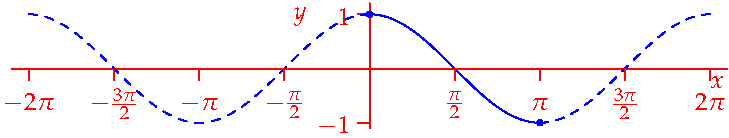
\includegraphics[width=\textwidth]{invcos2}\\
% $f(x)=\cos x$ is 1--1 on domain $[0,\pi]$\\[8pt]
% Inverse function $f^{-1}(x)=\arccos x=\cos^{-1}x$\\[8pt]
% Domain $\dom(\arccos)=[-1,1]$\\[8pt]
% Range $\operatorname{range}(\arccos)=[0,\pi]$\\
% \end{minipage}\qquad\begin{minipage}{0.4\textwidth}
% 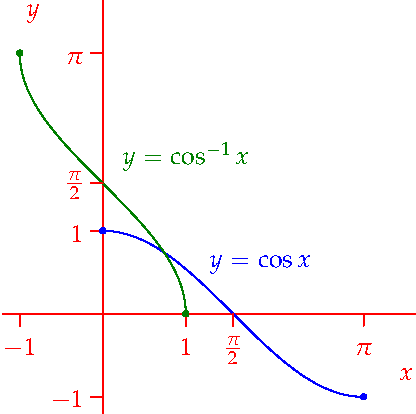
\includegraphics[width=\textwidth]{invcos}
% \end{minipage}\vspace{10pt}
% 
% \noindent\begin{minipage}{0.56\textwidth}
% 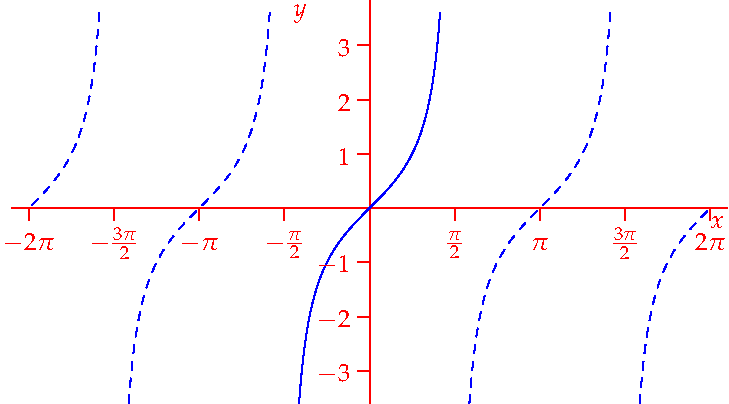
\includegraphics[width=\textwidth]{invtan2}\\
% $f(x)=\tan x$ is 1--1 on domain $(-\frac\pi 2,\frac\pi 2)$\\[8pt]
% Inverse function $f^{-1}(x)=\arctan x=\tan^{-1}x$\\[8pt]
% Domain $\dom(\arctan)=\R$\\[8pt]
% Range $\operatorname{range}(\arcsin)=(-\frac\pi 2,\frac\pi 2)$\\
% \end{minipage}\qquad\begin{minipage}{0.4\textwidth}
% 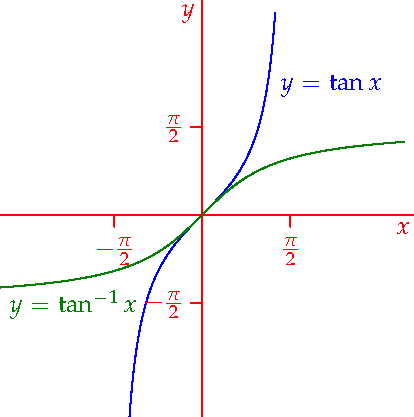
\includegraphics[width=\textwidth]{invtan}
% \end{minipage}


\subsection{Solving Triangles}

Basic trigonometry often involves finding the edges and angles of a triangle given partial data.

\begin{example}{}{easytree}
	To find the height $h$ of a tall tree, two angles of elevation \ang{45} and \ang{30} are measured a distance 20 ft apart along a straight line from the base of the trunk.\smallbreak
	This is easily attacked by drawing a picture and observing that we have two right-triangles. If the (unknown) distance from the base of the tree to the nearer measurement is $x$, then\par
	\begin{minipage}[t]{0.54\linewidth}\vspace{-7pt}
		\[
			\frac 1{\sqrt 3}=\tan\ang{30}=\frac h{x+20}\qquad 1=\tan\ang{45}=\frac hx
		\]
		Substituting the second equation into the first returns
		\[
			h=\frac{20}{\sqrt 3-1}\approx 27.32\,\text{ft}
		\]
	\end{minipage}
	\hfill
	\begin{minipage}[t]{0.45\linewidth}\vspace{-12pt}
		\flushright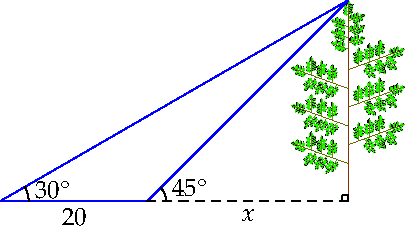
\includegraphics{tree2}
	\end{minipage}\smallbreak
		In fact there is enough data in the problem to recover everything about the \textcolor{blue}{original triangle.}
	\begin{itemize}\itemsep2pt
	  \item The second base angle is ($\ang{180}-\ang{45}=\ang{135}$).
	  \item The third (summit) angle is $\ang{180}-\ang{30}-\ang{135}=\ang{15}$.
	  \item Two applications of Pythagoras compute the remaining sides of the triangle
	  \begin{gather*}
	  	\sqrt{x^2+h^2}=\sqrt 2h=\frac{20\sqrt 2}{\sqrt 3-1}\approx 38.64\\
	  	\sqrt{h^2+(x+20)^2}=\sqrt{h^2+3h^2}=2h=\frac{40}{\sqrt 3-1}\approx 54.64
	  \end{gather*}
	\end{itemize}
\end{example}

\begin{minipage}[t]{0.7\textwidth}\vspace{-5pt}
	The example is just a disguised version of \emph{solving a triangle}: computing all six sides and angles of a triangle given three of them. The Euclidean triangle congruence theorems tell us which combinations are sufficient to determine all the others. The example is the ASA congruence: angle-side-angle data (\ang{30}--20--\ang{135}) is enough to compute everything else about the triangle.
\end{minipage}
\hfill
\begin{minipage}[t]{0.29\textwidth}\vspace{-10pt}
	\flushright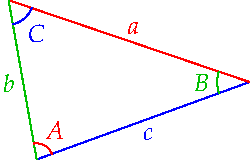
\includegraphics{euler}
\end{minipage}\medbreak

When in doubt, you can always attack basic trigonometry problems as we did in the example: create a right-triangle, then use the definitions of sin/cos/tan and/or Pythagoras.

\begin{example}{}{saseasy}
	Given the SAS (side-angle-side) combination 5--\ang{60}--9, find the third side of the triangle.\par
	\begin{minipage}[t]{0.7\textwidth}\vspace{-5pt}
		The altitude $h$ creates two right-triangles, from which
		\begin{gather*}
			h=5\sin\ang{60},\quad x=5\cos\ang{60}\\[5pt]
			\begin{aligned}
				\implies c^2&=(9-x)^2+h^2=9^2+(x^2+h^2)-18x\\
				&=9^2+5^2-18\cdot 5\cos\ang{60}=61
			\end{aligned}\\
			\implies c=\sqrt{61} \approx 7.81
		\end{gather*}
	\end{minipage}
	\hfill
	\begin{minipage}[t]{0.29\textwidth}\vspace{0pt}
		\flushright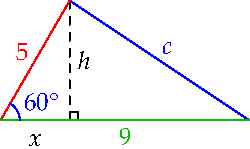
\includegraphics{exsas2}
	\end{minipage}\medbreak
	Since we now know $c$ and $9-x=\frac{13}2$ the remaining angles could also be easily found.
\end{example}
\goodbreak


In elementary situations it is typically easier to have students drop the perpendicular as we've done. However, once comfortable with the method, it is helpful to have short-cuts which skip the need to work with the perpendicular at all.


\begin{thm}{Sine and Cosine Rules}{}
	For any triangle,
	\[
		\frac{\sin A}a=\frac{\sin B}b=\frac{\sin C}c\ \ \text{ and }\ \ c^2=a^2+b^2-2ab\cos C
	\]
\end{thm}

The cosine rule is just the Pythagorean Theorem with a correction for non-right triangles. Both rules follow straightforwardly by drawing an altitude as before!

\begin{proof}
	Consider the picture. We have\par
	\begin{minipage}[t]{0.6\linewidth}\vspace{-11pt}
		\[
			h=a\sin C=c\sin A,\quad x=a\cos C,\quad b-x=c\cos A
		\]
		The first equation rearranges to
		\[
			\frac{\sin A}a=\frac{\sin C}c
		\]
		Two applications of Pythagoras give the cosine rule
	\end{minipage}
	\hfill
	\begin{minipage}[t]{0.39\linewidth}\vspace{-5pt}
		\flushright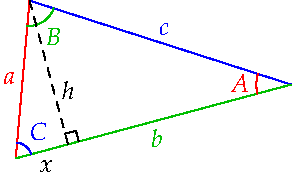
\includegraphics{sinerule}
	\end{minipage}\smallbreak
	\[
		c^2=h^2+(b-x)^2=h^2+x^2+b^2-2bx =a^2+b^2-2ab\cos C
	\]
	The remaining part of the sine rule and the other versions of the cosine rule are obtained by choosing other altitudes.
\end{proof}


Here are two examples where we use the rules instead of explicitly drawing an altitude.

\begin{examples}{}{}
	\exstart A triangle has sides 2 and $\sqrt 3-1$, and the angle between them is \ang{120}. Find the remaining sides and angles.%\par
	\begin{enumerate}\setcounter{enumi}{1}
		\item[] We apply the cosine rule with $\textcolor{red}{a=2}$, $\textcolor{Green}{b=\sqrt 3-1}$ and $\textcolor{blue}{C=\ang{120}}$\par
		\begin{minipage}[t]{0.79\linewidth}\vspace{-20pt}
		  \begin{align*}
		    c^2&=a^2+b^2-2ab\cos C\\
		    &=2^2+(\sqrt 3-1)^2-2\cdot 2(\sqrt 3-1)\cos\ang{120} \\
		    &=4+3+1-2\sqrt 3+2(\sqrt 3-1) =6
		  \end{align*}
		  We have an opposite pair $(\textcolor{blue}{c},\textcolor{blue}{C})=(\textcolor{blue}{\sqrt 6},\textcolor{blue}{\ang{120}})$, so the sine rule may be used
		  \[
		  	\sin A=\frac 2{\sqrt 6}\sin\ang{120}=\frac{2\sqrt 3}{2\sqrt 6}=\frac 1{\sqrt 2}\implies \textcolor{red}{A=\ang{45}}
		  \]
		  We chose the acute angle since $A=\ang{180}-B-C=\ang{60}-B<\ang{90}$.\smallbreak
		  The final angle is then $\textcolor{Green}{B}=\ang{180}-\textcolor{red}{\ang{45}}-\textcolor{blue}{\ang{120}}=\textcolor{Green}{\ang{15}}$.
		\end{minipage}
		\hfill
		\begin{minipage}[t]{0.2\linewidth}\vspace{-28pt}
			\flushright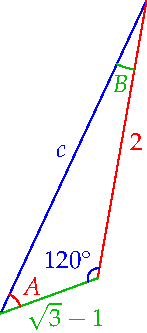
\includegraphics{exsas}
		\end{minipage}\smallbreak
		
		You could instead drop a perpendicular, say from the vertex $A$ to the \emph{extension} of the side of length 2. Think about why the perpendicular has to be \emph{outside} the triangle\ldots

		\goodbreak
		
		\item A triangle has one side with length 5 and its two adjacent angles are \ang{40} and \ang{65}. Find the remaining data.\par
		\begin{minipage}[t]{0.69\linewidth}\vspace{-5pt}
			This time the initial data is ASA. Writing $\textcolor{blue}{c=5}$, $\textcolor{red}{A=\ang{40}}$ and $\textcolor{Green}{B=\ang{65}}$, the remaining angle is plainly 
			\[
				\textcolor{blue}{C}=\ang{180}-\textcolor{red}{\ang{40}}-\textcolor{Green}{\ang{65}}=\textcolor{blue}{\ang{75}}
			\]
			This gives us an opposite pair $(\textcolor{blue}{c,C})$, so we can apply the sine rule
			\[
				\textcolor{red}{a}=c\,\frac{\sin A}{\sin C}=\textcolor{blue}{5}\,\frac{\sin\textcolor{red}{\ang{40}}}{\sin\textcolor{blue}{\ang{75}}}\approx 3.327
			\]
			A second application yields
			\[
				b=c\,\frac{\sin B}{\sin c}=\textcolor{blue}{5}\,\frac{\sin\textcolor{Green}{\ang{65}}}{\sin\textcolor{blue}{\ang{75}}}\approx 4.691
			\]
		\end{minipage}
		\hfill
		\begin{minipage}[t]{0.3\linewidth}\vspace{-5pt}
			\flushright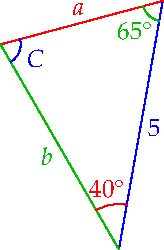
\includegraphics{exasa}
		\end{minipage}
	\end{enumerate}
\end{examples}



\begin{minipage}[t]{0.6\textwidth}\vspace{0pt}
	\boldsubsubsection{Multiple-angle Formulae}
	Also useful in the context of basic trigonometry is the ability to sum angles. The picture provides a simple justification of
	\[
		\sin(\alpha+\beta)=\textcolor{Green}{\sin\alpha\cos\beta} + \textcolor{blue}{\cos\alpha\sin\beta}
	\]
	at least when $0<\alpha+\beta<\frac\pi 2$. If you look carefully, you should be able to see how the same picture establishes
	\[
		\cos(\alpha+\beta)=\cos\alpha\cos\beta - \sin\alpha\sin\beta
	\]
\end{minipage}
\hfill
\begin{minipage}[t]{0.39\textwidth}\vspace{0pt}
	\flushright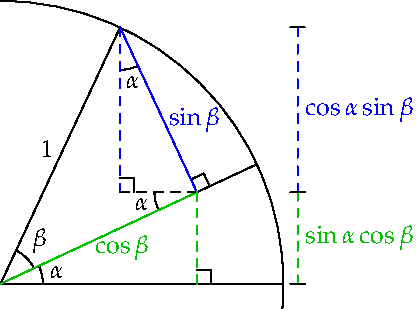
\includegraphics[scale=0.85]{multipleangle}
\end{minipage}

\vfil

  
\begin{exercises}{}{}
	\exstart Find the remaining angles in the triangle in Example \ref{ex:saseasy}; you'll need a calculator to convert to degrees.
	\begin{enumerate}\setcounter{enumi}{1}
	  \item The other Euclidean congruence theorems are SSS and SAA. Explain how to solve triangles using these minimal data in two ways:
	  \begin{enumerate}
	    \item By drawing an altitude.
	    \item Using the sine/cosine rules.
	  \end{enumerate}
	
	  \item SSA isn't a triangle congruence theorem. For instance, there are \emph{two} non-congruent triangles with data $a=1$, $b=\sqrt 3$ and $A=\ang{30}$. Find them.
	
	
	  \item Use the multiple-angle formulae to derive the familiar expressions for $\sin 2\theta$ and $\cos 2\theta$.
	  
	  \item Find the exact value of $\sin\ang{105}$.
	  
	  \item\begin{enumerate}
	    \item Find an expression for $\tan(\alpha+\beta)$ purely in terms of $\tan\alpha$ and $\tan\beta$.
	  	 \item Two wooden wedges with slope $\frac 14$ are placed on top of each other to make a steeper slope. What is the gradient of the new slope?
	  \end{enumerate} 
	\end{enumerate}
\end{exercises}


\clearpage


\subsection{Polar Co-ordinates}

Definition \ref{defn:polarcoord} provides an alternative way to describe points in the plane. If $\theta$ is the polar angle of a point with Cartesian (rectangular) co-ordinates $(x,y)$, then its polar-coordinates are precisely the values $(r,\theta)$ seen in the definition!\smallbreak

Computing $x=r\cos\theta$ and $y=r\sin\theta$ is easy given $r$ and $\theta$.

\begin{example}{}{polar}
	A point with polar co-ordinates $\textcolor{blue}{(r,\theta)=(2,\frac{5\pi}6)}$ has Cartesian co-ordinates
	\[
		\textcolor{blue}{(x,y)=\bigl(2\cos\tfrac{5\pi}6,2\sin\tfrac{5\pi}6\bigr) =\bigl(-\sqrt 3,1\bigr)}
	\]
\end{example}

Computing polar co-ordinates from Cartesian is harder, requiring some \emph{visualization.}  
\begin{enumerate}
  \item Every point $(x,y)$ has a unique radius $r=\sqrt{x^2+y^2}$, but not polar angle. If $\theta$ is a polar angle, so is $\theta+2\pi n$ for any integer $n\in\Z$. The origin $(x,y)=(0,0)$ is even stranger; certainly $r=0$, but \emph{any} $\theta$ is a legitimate polar angle!
  \item Whenever $x\neq 0$ (away from the $y$-axis),
  \[
  	\begin{cases}
  		x=r\cos\theta\\
  		y=r\sin\theta
  	\end{cases}
  	\implies \tan\theta=\frac yx
  \]
	however, this \emph{doesn't} guarantee that $\theta=\tan^{-1}\frac yx$. Continuing the example shows us why\ldots
\end{enumerate}

\begin{example*}[lower separated=false, sidebyside, sidebyside align=top seam, sidebyside gap=0pt, righthand width=0.35\linewidth]{\ref{ex:polar}, cont}{}
	If $\textcolor{blue}{(x,y)=(-\sqrt 3,1)}$, then the radius is easy
	\[
		r=\sqrt{(\sqrt 3)^2+1^2}=2
	\]
	For the polar angle,
	\[
		\tan\theta=\frac yx=-\frac 1{\sqrt 3}=\tan\left(-\frac\pi 6\right)\notimplies \theta=\textcolor{orange}{-\frac\pi 6}
	\]
	Arctan has range $(-\frac\pi 2,\frac\pi 2)$, so always returns an angle in quadrants 1 or 4. Our point is in the \emph{second} quadrant ($x<0<y$) so we need to adjust, using the fact that $\tan$ is $\pi$-periodic:
	\[
		\textcolor{blue}{\theta=\pi-\frac\pi 6=\frac{5\pi}6} =\ang{150}
	\]
	We could alternatively add any integer multiple of $2\pi$.
	\tcblower
	\flushright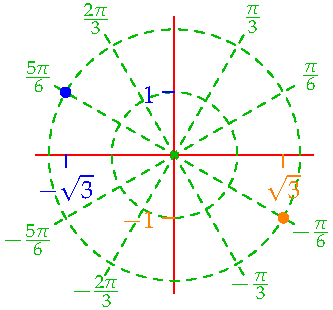
\includegraphics{expolar}
\end{example*}


The example wasn't too tricky since the polar angle was exactly computable. When you have to rely on a calculator, it is much easier to make a mistake.

\begin{example}{}{}
	The point $(x,y)=(-8,-15)$ has polar co-ordinates (quadrant 3!)
	\[
		r=\sqrt{8^2+15^2}=17,\qquad \theta=\pi+\tan^{-1}\tfrac{15}8\approx \ang{241.93}
	\]
\end{example}


We could summarize with formulæ describing precisely how to compute $\theta$ dependent on quadrant (the signs of $x,y$), though it is better to get in to the habit of drawing a picture!

\goodbreak


\boldsubsubsection{Curves in Polar Co-ordinates}

Polar co-ordinates are well-suited to describing curves that encircle the origin. Indeed circles centered at the origin with radius $a>0$ have the very simple polar form $r=a$. Converting to rectangular co-ordinates recovers the the natural parametrization of a circle:
\[
	x(\theta)=a\cos\theta,\quad y(\theta)=a\sin\theta
\]
This partly explains why mathematicians call sine and cosine \emph{circular functions.}\smallbreak

General polar graphs are harder to visualize, though the major reason is lack of familiarity. Have a little empathy: to graph \emph{polar} functions, you'll likely have to follow the same approach as new students use to sketch \emph{Cartesian} curves like $y=x^2$! Here are a couple of examples.

\begin{examples}{}{}
	\exstart The curve $r=\theta$ is relatively easy to plot since $r$ increases at exactly the same rate as the angle; we therefore have a \emph{spiral.}\vspace{-5pt}
	\begin{enumerate}\setcounter{enumi}{1}
	  \item[]To confirm this, plot several points $(\theta,\theta)$; we've done for $\theta$ in multiples of $\frac\pi 6$ \ ($\ang{30}$) from 0 to $2\pi$. It is sensible to use `polar graph paper' with concentric circles separated by (say) $\frac\pi 2\approx 1.57$.
	  \begin{center}
	  	\begin{tabular}{c@{\qquad\qquad}c}
	  		\begin{tabular}{c}
	  			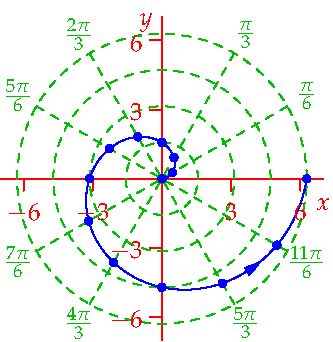
\includegraphics{expolar2}
	  			\\
	  			$r=\theta$, \ $0\le \theta\le 2\pi$
	  		\end{tabular}
	  		&
	  		\begin{tabular}{c}
	  			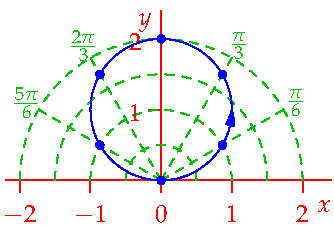
\includegraphics{expolar3}
	  			\\
	  			$r=2\sin\theta$, \ $0\le \theta\le\pi$
	  			\\[8pt]
	  			$\def\arraystretch{1.2}
	  			\begin{array}{|c|cccccc|}\hline
						\theta&\frac\pi 6&\frac{2\pi}3&\frac\pi 2&\frac{4\pi}3&\frac{5\pi}6&\pi\\\hline
						2\sin\theta&1&1.73&1&1.73&1&0\\\hline
					\end{array}$
	  		\end{tabular}
	  	\end{tabular}
	  \end{center}
	  
	  \item The curve $r=2\sin\theta$ is a little easier to work with since we know exact values for sine, assisted by $\sqrt 3\approx 1.73$.\par
		This looks like a circle! To see this, multiply both sides by $r$ and complete the square:
		\[
			r^2=2r\sin\theta\implies x^2+y^2=2y \implies x^2+(y-1)^2=1
		\]
		describes the set of points with distance 1 from the point $(0,1)$: a circle!
	\end{enumerate}
\end{examples}

You should think about what happens in both examples if we extend the domain:
\begin{itemize}
  \item What would $r=\theta$ look like if $\theta$ were allowed to be \emph{negative}?
  \item What happens to $r=2\sin\theta$ when $\theta>\pi$? 
\end{itemize}


\clearpage


\begin{exercises}{}{}
	\exstart Convert the following points to polar co-ordinates.
	\begin{enumerate}\setcounter{enumi}{1}
	  \item[]\begin{enumerate}
	    \item $(-5,5)$\qquad (b)\lstsp $(3,-4)$\qquad (c)\lstsp $(-5\sqrt 3,-15)$
	    \item[(d)] $(-1,\tan 3)$\quad (tricky---this is 3 radians!)
	  \end{enumerate}
	  
	  \item If $a>0$, describe the curve with polar equation $r=2a\cos\theta$.\par
	  (\emph{Be careful with $\theta>\frac\pi 2$ since cosine goes negative\ldots})
	  
	  \item The algebraic trickery in the last example sometimes bears fruit, though you have to be lucky! By multiplying both sides by $1-\sin\theta$ and converting to rectangular co-ordinates, show that the polar function
		\[
			r(\theta)=\frac{2a}{1-\sin\theta}
		\]
		is a parabola in disguise and sketch it when $a=1$. How does the graph depend on $a$?
		 
	  \item Try to sketch the following curves.
		\begin{enumerate}
	  	\item $r=\theta(\theta-4)$\qquad (b)\lstsp $r=(\theta-1)^2+1$\qquad (c)\lstsp $r=(\theta-1)^2-1$
		\end{enumerate}
		As well as plotting points directly, you should sketch the curve first on rectangular axes (e.g.,{} (a) is $y=x(x-4)$). What happens to (c) when $\theta=1$?\par
		Once you've tried these, use a \href{https://www.desmos.com/calculator}{grapher} to see if you're right, though see how close you can get without it! 
	\end{enumerate}
\end{exercises}


\iffalse
\begin{minipage}[t]{0.7\linewidth}\vspace{0pt}
\boldinline{Conics in Polar Co-ordinates}

A fun application is to recover polar forms for the standard conics. We use the focus/directrix/eccentricity definition, place the origin at a focus $F$ and directrix $d$ vertically to the right of the origin. Recall that a conic with eccentricity $e$ may be described as the set of points $P$ such that $\nm{PF}=e\nm{Pd}$. Exactly one point on the conic ($K$) lies between the focus and directrix. If we let $\nm{KF}=k$, it should be clear from the picture that
\[\frac re+r\cos\theta=k+\frac ke \implies r=\frac{k(1+e)}{1+e\cos\theta}\]
This is \emph{independent} of the type of conic, and even works when $e=0$; $r=2k$ is a circle with radius $k$!
\end{minipage}\begin{minipage}[t]{0.3\linewidth}\vspace{0pt}
\flushright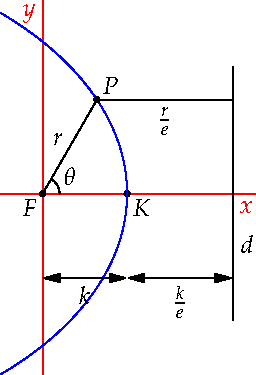
\includegraphics{eccentric}
\end{minipage}

\begin{itemize}
  \item If $e<0$, then $1+e\cos\theta>0$ for all $\theta$ and $r$ is always defined. We obtain a closed curve: an ellipse.
  \item If $e=1$, then $1+\cos\theta=0$ when $\theta=\pi$. We obtain a parabola opening leftwards.
  \item If $e>1$, then $1+e\cos\theta=0$ at two values $\theta=\pm\cos^{-1}\frac 1e$. These lines are parallel to the asymptotes of the hyperbola. Permitting $r<0$, the remaining values of $\theta$ give the other branch of the hyperbola!
\end{itemize}


\begin{exercises}{}{}
\def\hvr{\hat{\vr}}
\def\hth{\hat{\pmb\theta}}
\hangindent\leftmargini
\textup{1. } If $e=1$, find the \emph{rectangular} equation of the parabola described by the above.
\begin{enumerate}\setcounter{enumi}{1}
  \item (If you know a little Physics\ldots)\quad Let $\hvr=\stwovec{\cos\theta}{\sin\theta}$ be the unit vector pointing away from the origin, and $\hth=\stwovec{-\sin\theta}{\cos\theta}$ be the unit vector obtained by rotating $\hvr$ counter-clockwise by \ang{90}.
  \begin{enumerate}
    \item Check that $\diff t\hvr=\dot r\hth$, where $\dot r=\diff[r]{t}$ means differentiation with respect to time. What is $\diff t\hth$ in terms of $\hvr$?
    \item Verify that
    \[\diff[^2]{t^2}(r\hvr) =(\ddot r-r\dot\theta^2)\hvr+\frac 1r\left[\diff t(r^2\dot\theta)\right]\hth\]
    \item Note that $r\hvr$ is the position vector of a point with polar co-ordinates $(r,\theta)$. If an inverse-square attractive \emph{force} acts on a particle, Newton's second law tells use that
    \[\diff[^2]{t^2}(r\hvr) =-\frac b{r^2}\hvr\]
    for some positive constant $b$. This is Newton's model of gravity.\par
    Check that \emph{every conic} is a solution to this differential equation.\par
    (\emph{Hint: use the fact that $r^2\dot\theta$ is constant! This is essentially conservation of angular momentum}) 
  \end{enumerate}
  This explains Kepler's 1\st\ law, that planets orbit the sun in ellipses with the sun at one focus. The other conical orbits are indeed possible: comets regularly pass the sun along hyperbolic orbits, never to return to the solar system.
\end{enumerate}
\end{exercises}


\fi

% Curves in polar co-ordinates
% 
% Polar co-ordinates and conics?
% 
% Put focus at center; $\nm{PF}=e\nm{PQ}\implies r=e(r\sin\theta+1)=a(e+1)\implies r=\frac{a(1+e)}{1+e\sin\theta}$
% 
% 
% 
% Angle of cone/plane gives eccentricity.

% AFTER MIDTERM: conic sections. Parabola, ellipse and hyperbola old-school style. reflections, etc. Mirror. Planet orbits? Gauss and regression/normal distribution.

